\documentclass{article}
%%%%%%%%%%%%%%%%%
%%%%%%%%%%%%%%%%%%
\author{Matthew Bates}
\usepackage{xfrac}
\usepackage{amsmath}
\usepackage{fancyhdr}
\usepackage{gensymb}
\linespread{0.7}
\usepackage{graphicx}
\usepackage{subcaption}
\usepackage[font = footnotesize]{caption}
\usepackage{wrapfig}
\graphicspath{{C:/Users/Matt/Workshop/DataVis/Assignment2/Images/}}
\usepackage[parfill]{parskip}
\usepackage{geometry}
\usepackage{hyperref}
\usepackage{breakcites}
\usepackage{listings}
%%%%%%%%%%%%%%%%%%%
\geometry{
a4paper,
total={150mm,237mm},
left = 30mm,
top = 30mm,
}
%%%%%%%%%%%%%%%%%%%
\hypersetup{
    colorlinks=false,
    pdfborder={0 0 0},
}
%%%%%%%%%%%%%%%%%%%
\pagestyle{fancy}
\lhead{Matthew Bates}
\rhead{CSCM37 - Data Visualisation}
\chead{Assignment One}
%%%%%%%%%%%%%%%%%%%
%%%%%%%%%%%%%%%%%%%

\begin{document}
\begin{titlepage}
    \begin{center}
        \vspace*{1cm}
        
	\Huge
        \textbf{Assignment Two - Volume Visualization}
        
        \vspace{0.5cm}
	\LARGE
        Volume Data Conversion and Discovery
         \vfill

	CSCM37 - Data Visualisation - Robert S. Laramee\\
	Department of Computer Science\\
	Swansea University\\
 	Wales, UK
        \vspace{1.5cm}
	\begin{figure}[h]
    		\centering
    		\begin{subfigure}[b]{0.3\textwidth}
        		\includegraphics[width=\textwidth]{/../../../Bureacracy/SwanseaLogo.jpg}
    		\end{subfigure}
		\begin{subfigure}[b]{0.215\textwidth}
        		\includegraphics[width=\textwidth]{/../../../Bureacracy/CardiffLogo.jpg}
        	\end{subfigure}
	\end{figure}
        

        
        \vspace{0.8cm}
        \Large
        \textbf{Matthew Bates}\\
        School of Physics and Astronomy\\
        Cardiff University\\
        Wales, UK\\
        23 March, 2018
        
    \end{center}
\end{titlepage}

\pagenumbering{arabic}

\section{Sample Data Set from Paraview: Heating of Air due to a hot, rotating Disk}
\subsection{Visualising the Air Currents above the Disk.}
\begin{figure}[h]
	\centering
	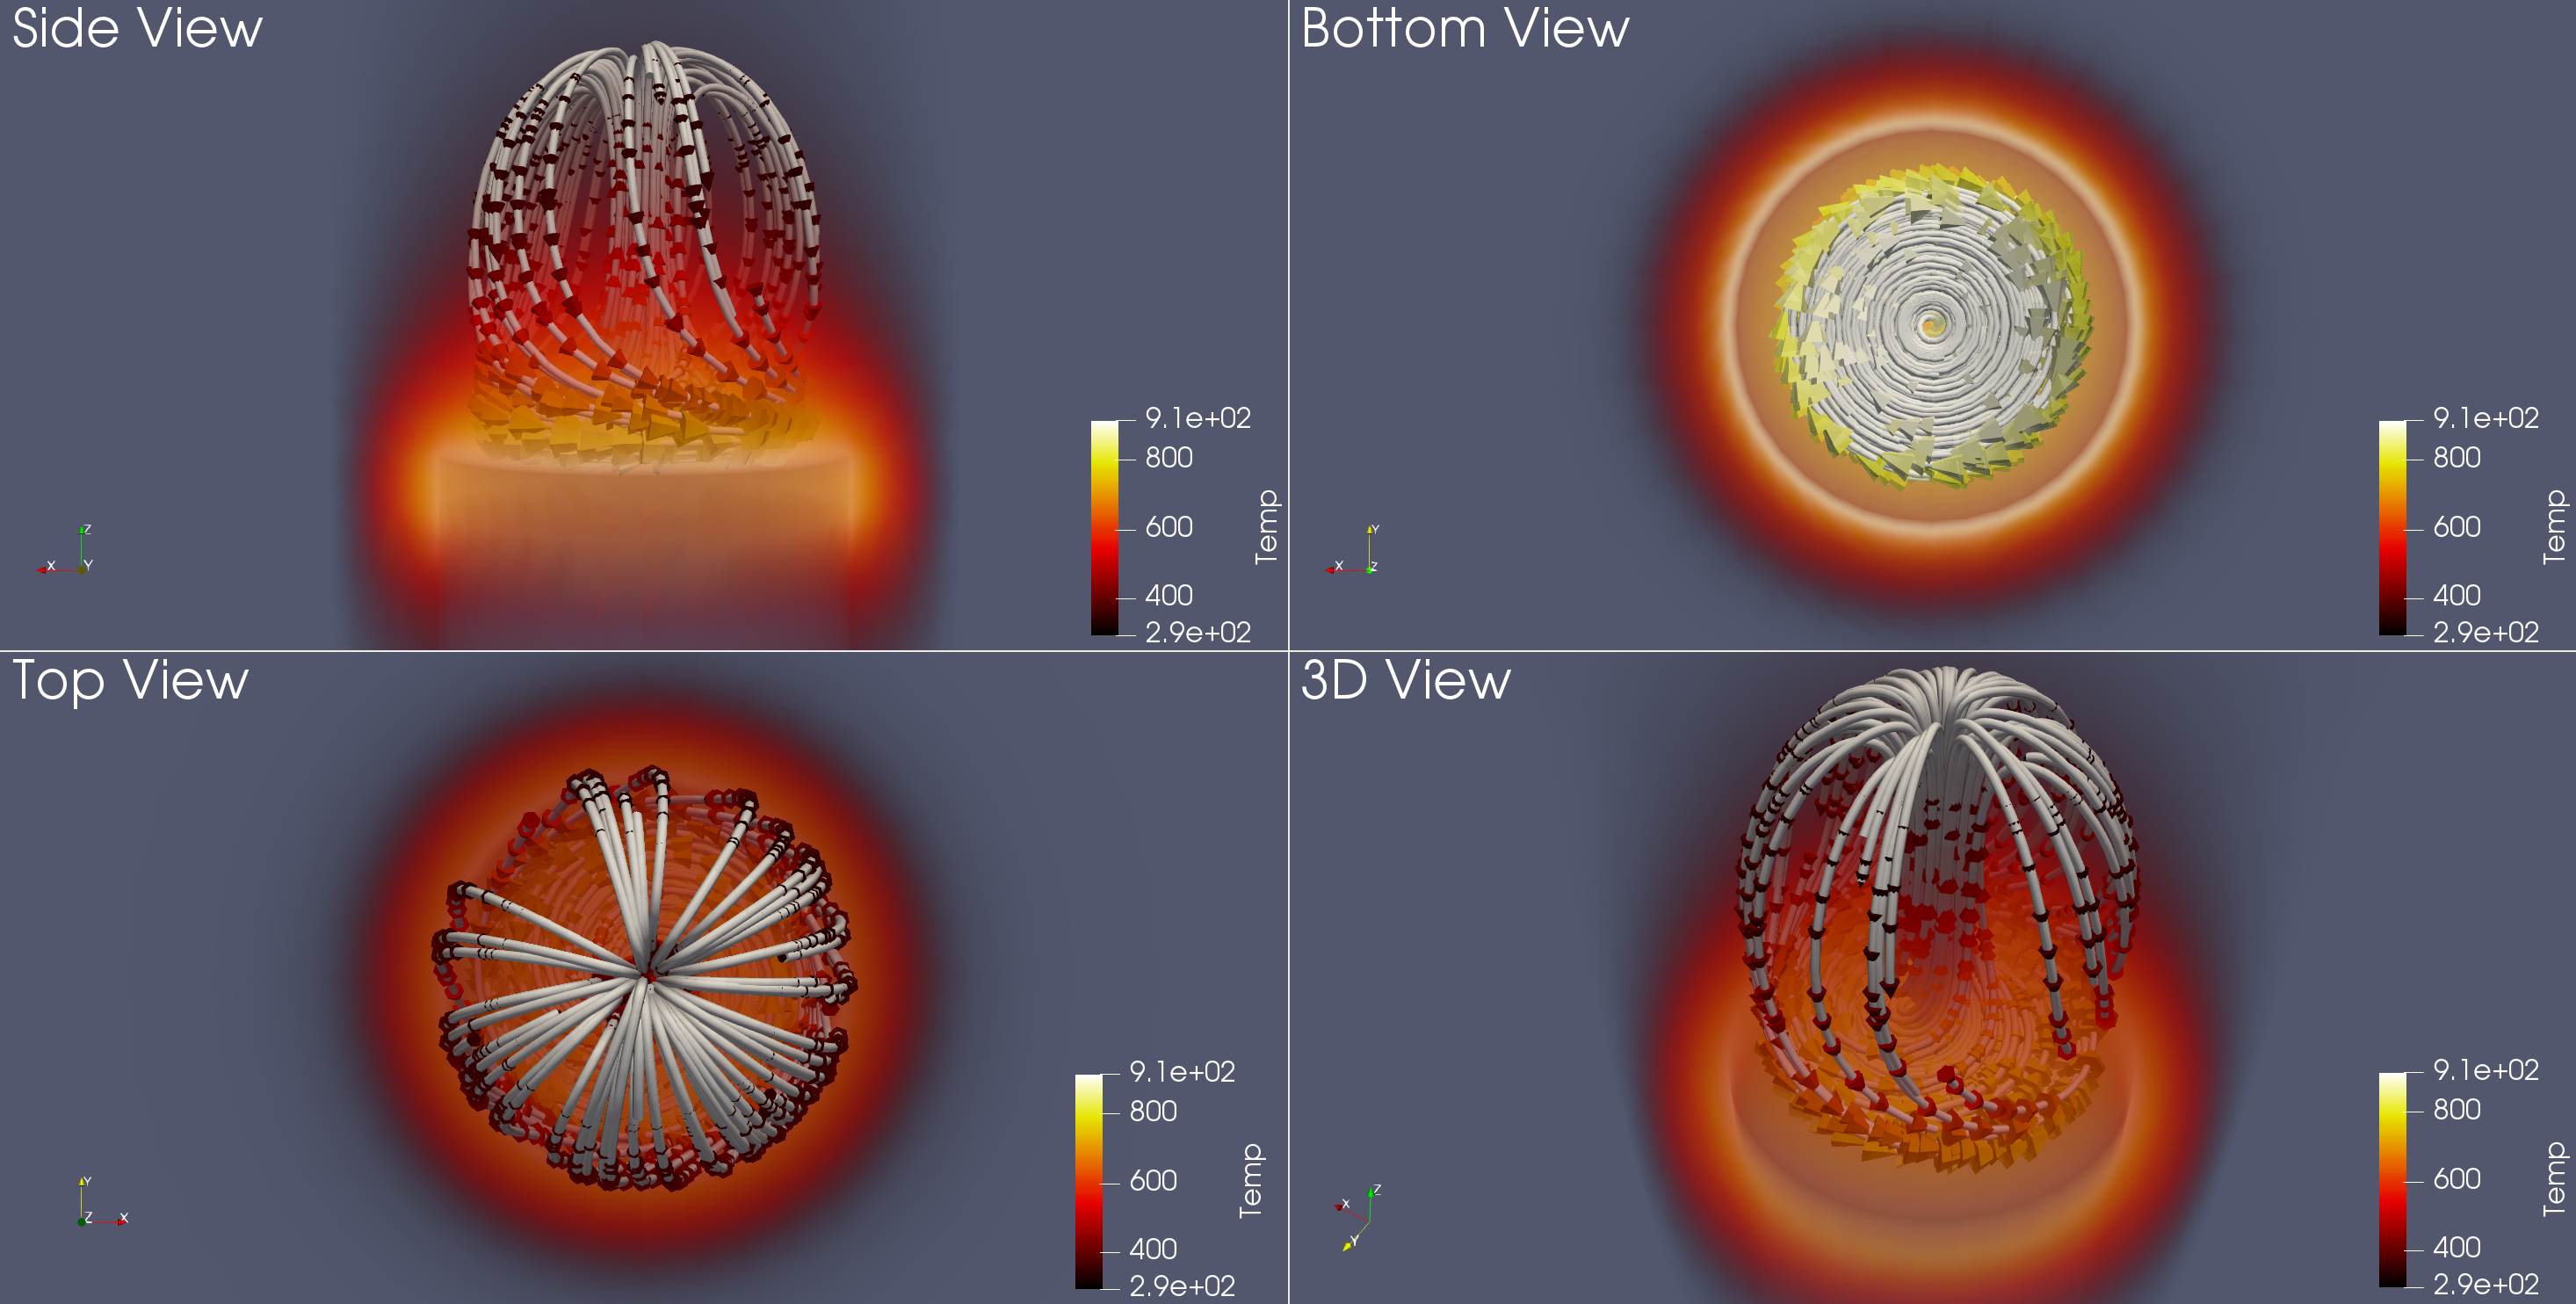
\includegraphics[width=\linewidth]{Section11.png}
\end{figure}
\begin{description}
	\item[$\bullet$ Tool:] ParaView 5.50
	\item[$\bullet$ Visualisation Type:] A
	\item[$\bullet$ Visual Mappings:] \hfill
		\begin{description}
			\item[$-$ colour:] A
			\item[$-$ size:] A
			\item[$-$ position:] A
		\end{description}
	\item[$\bullet$ Unique Observation:] A
\end{description}
\newpage

\subsection{Temperature and Pressure Variation around the Disk}
\begin{figure}[h]
	\centering
	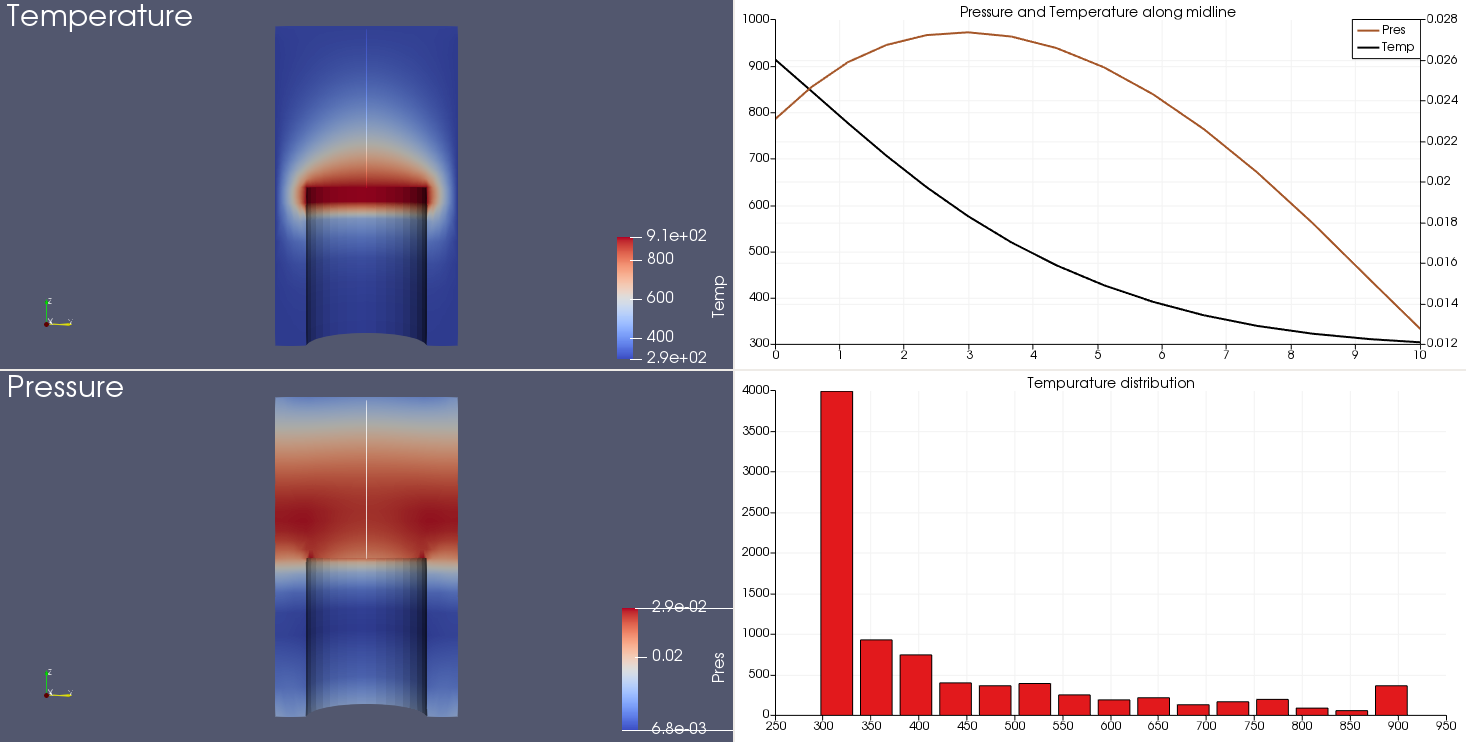
\includegraphics[width=\linewidth]{Section12.png}
\end{figure}
\begin{description}
	\item[$\bullet$ Tool:] ParaView 5.50
	\item[$\bullet$ Visualisation Type:] A
	\item[$\bullet$ Visual Mappings:] \hfill
		\begin{description}
			\item[$-$ colour:] A
			\item[$-$ size:] A
			\item[$-$ position:] A
		\end{description}
	\item[$\bullet$ Unique Observation:] A
\end{description}
\newpage

\section{Sally}
\subsection{Velocity Visualisation}
\begin{figure}[h]
	\centering
	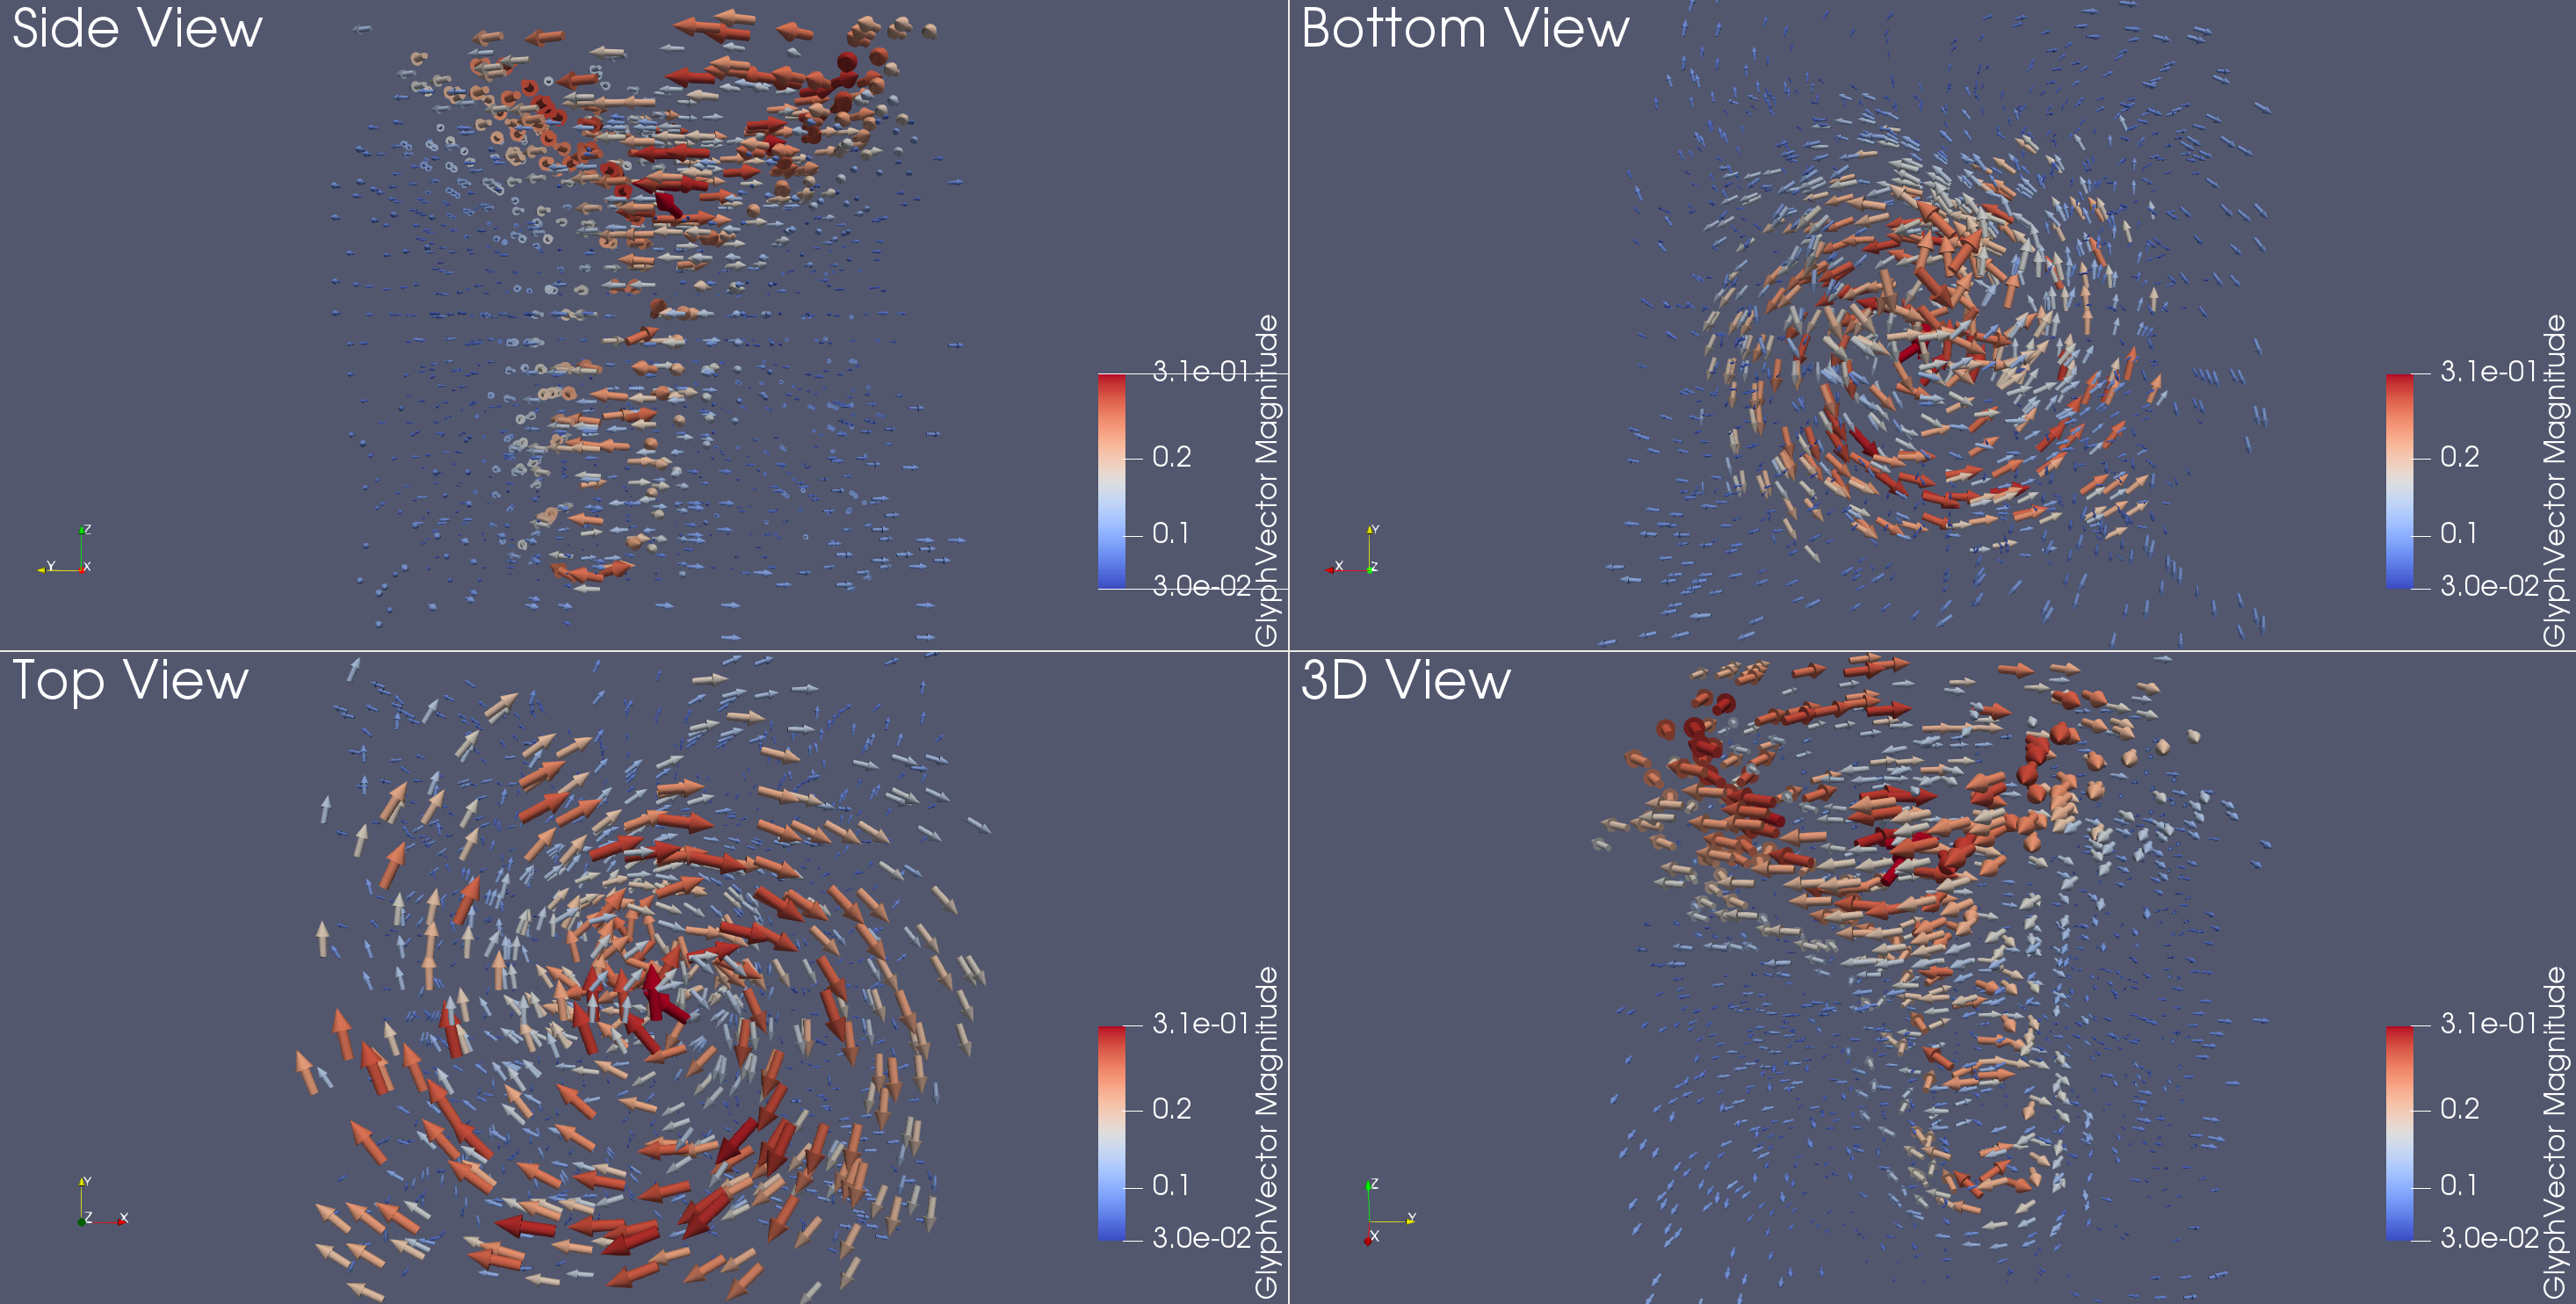
\includegraphics[width=\linewidth]{Section21.png}
\end{figure}
\begin{description}
	\item[$\bullet$ Tool:] ParaView 5.50
	\item[$\bullet$ Visualisation Type:] A
	\item[$\bullet$ Visual Mappings:] \hfill
		\begin{description}
			\item[$-$ colour:] A
			\item[$-$ size:] A
			\item[$-$ position:] A
		\end{description}
	\item[$\bullet$ Unique Observation:] A
\end{description}
\newpage

\subsection{Tornado Animation}
\begin{figure}[h]
	\centering
	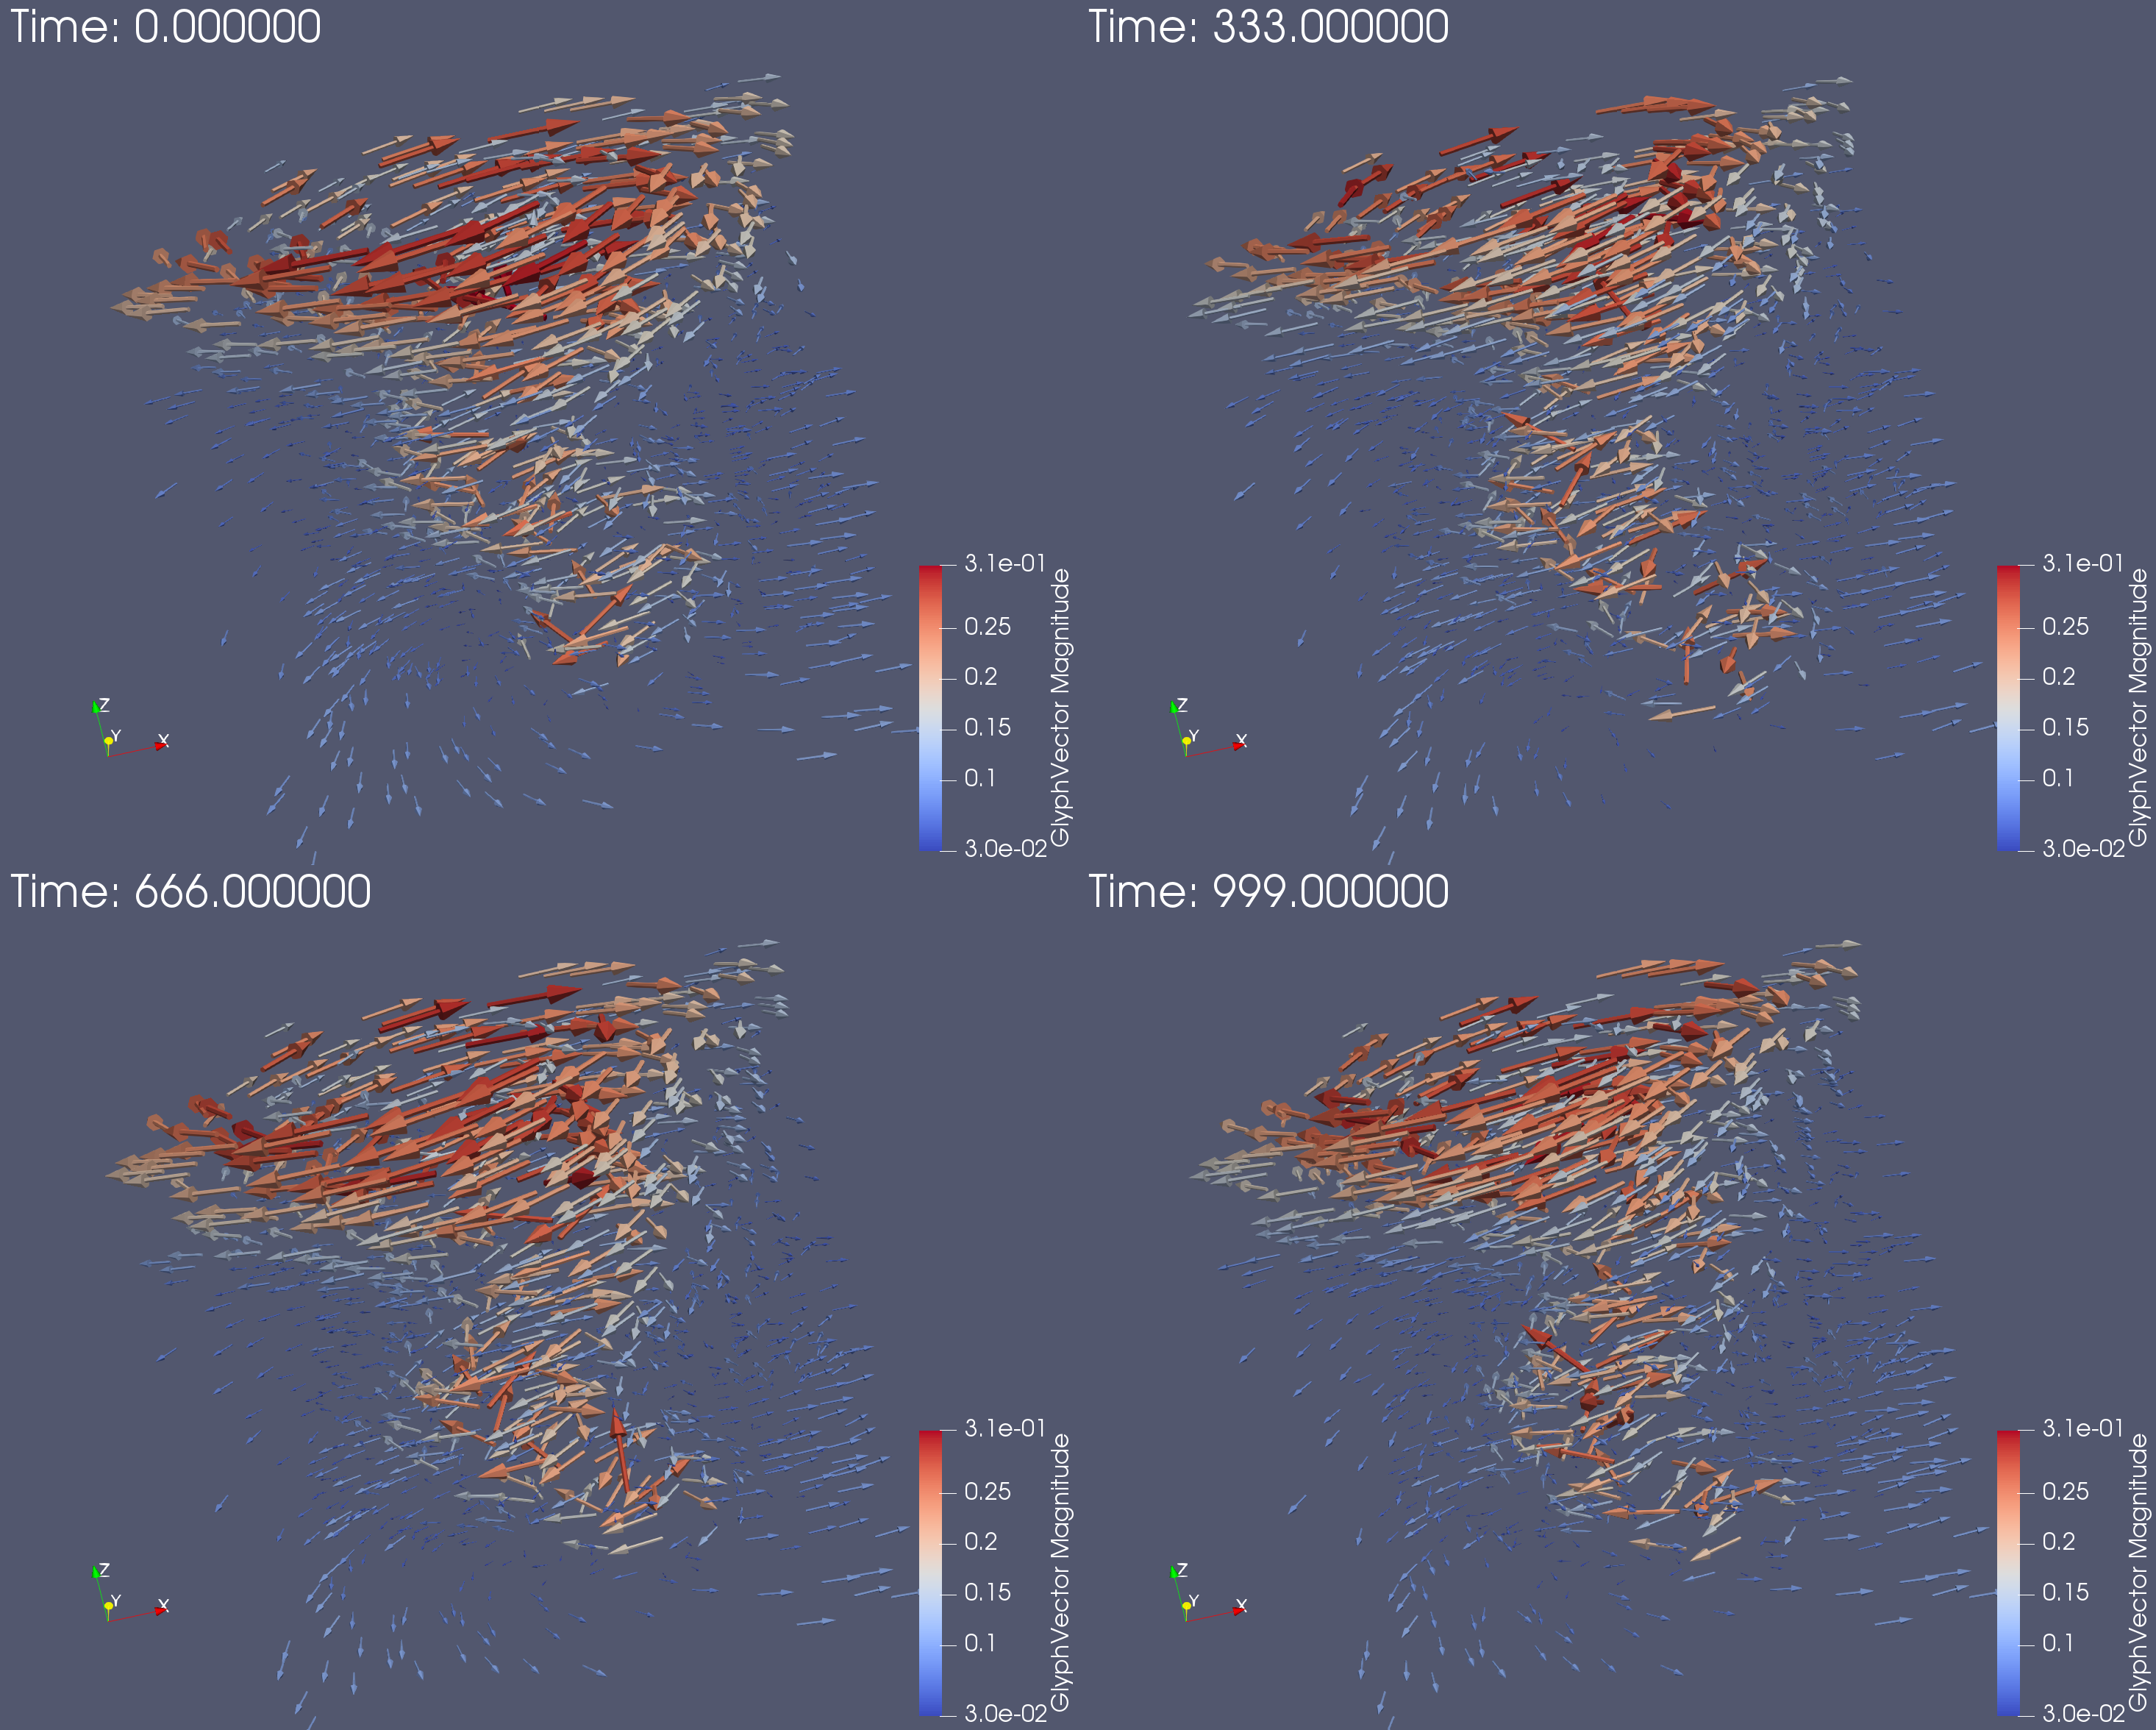
\includegraphics[width=\linewidth]{Section22.png}
\end{figure}
\begin{description}
	\item[$\bullet$ Tool:] ParaView 5.50
	\item[$\bullet$ Visualisation Type:] A
	\item[$\bullet$ Visual Mappings:] \hfill
		\begin{description}
			\item[$-$ colour:] A
			\item[$-$ size:] A
			\item[$-$ position:] A
		\end{description}
	\item[$\bullet$ Unique Observation:] A
\end{description}
\newpage

\end{document}